\documentclass[10pt,xcdraw]{article}

\usepackage[es-tabla]{babel}
\usepackage{parskip}
\usepackage[capitalise, noabbrev]{cleveref}
\crefname{table}{\spanishtablename}{\spanishtablename}



\title{
	\textbf{
		Desarrollo de un modelo fundacional estocástico basado en procesos Gaussianos para la clasificación de bioseñales EEG en el diagnóstico asistido del TDAH.
	}
	}
\author{
	Julián David Pastrana Cortés, M.Sc.
	}


\date{} % Carga el preámbulo
\begin{document}
	%%%%%%%%%%%%%%%%%%%%%%%%%%%%%%%%%% PORTADA %%%%%%%%%%%%%%%%%%%%%%%%%%%%%%%%%%%%%%%%%%%%
\vspace*{0.5cm}
\begin{center}
	\newcommand{\HRule}{\rule{\linewidth}{0.5mm}}
	\vspace*{-1.5cm}
	% \textsc{\huge Universidad Tecnológica\\ \vspace{5px} de Pereira}\\[1.5cm]
	% 
\includegraphics[width=0.2\textwidth]{imagenes/Logo_UTP.png}
	% \vspace{1.5cm}
	\textsc{\LARGE Informe de actividades en el marco del programa: \\ 
		\vspace{0.4cm}
		ALIANZA CIENTÍFICA CON ENFOQUE COMUNITARIO PARA MITIGAR BRECHAS DE ATENCIÓN Y MANEJO DE TRASTORNOS MENTALES RELACIONADOS CON IMPULSIVIDAD EN COLOMBIA
		}\\
	\vspace{2cm}
	\HRule \\[0.4cm]
	{ \bfseries Nombre: Julián David Pastrana Cortés }\\[0.4cm]
	{ \bfseries Contrato de servicios: 5551 }\\[0.4cm]
	\vspace{1.5cm}
	
\includegraphics[width=0.28\textwidth]{imagenes/LogoU.png}
	
\includegraphics[width=0.35\textwidth]{imagenes/logo_automatica.png}
	\HRule \\[1.5cm]
	\vspace{1.5cm}
	\vspace*{0.5cm}
	\textsc{\textbf{\Large Grupo de investigación en Automática } }\\
	\vspace{3.5cm} 
	\begin{center}
		{\large \today}
	\end{center}
\end{center}
\newpage
   % Carga la portada y otros elementos de layout
	
	\tableofcontents 
	\newpage
	
	\section{Información general del contrato}
	\begin{table}[H]
		\centering
		\begin{tabular}{>{\arraybackslash}m{8cm} >{\arraybackslash}m{6.5cm}}
			\toprule
			\textbf{Rol} & \vspace{2mm}Contratista - Estudiante de Doctorado\vspace{2mm}\\\hline
			\vspace{2mm}
			\textbf{Contrato de servicios No.}\vspace{2mm} & \vspace{2mm} 5551 de 2025\vspace{2mm}\\\hline
			\vspace{2mm}
			\textbf{Objeto del contrato} \vspace{2mm} & \vspace{2mm} Prestación de servicios profesionales para el Desarrollo de metodología de gamificación para entrenamiento de niños con trastornos de impulsividad ALIANZA CIENTÍFICA CON ENFOQUE COMUNITARIO PARA MITIGAR BRECHAS DE ATENCIÓN Y MANEJO DE TRASTORNOS MENTALES RELACIONADOS CON IMPULSIVIDAD EN COLOMBIA - ACEMATE MINCIENCIAS CONTRATO 790-2023 
			\vspace{2mm}\\\hline
			\textbf{Período del informe} & \vspace{2mm} 01 de marzo de 2025 al 31 de marzo de 2025\vspace{2mm}\\\hline
		\end{tabular}
	\end{table}
	
	\subsection{Descripción general de la vinculación}
	Como resultado de la vinculación se contribuye al alcance de el objetivo 3 del programa de investigación: ALIANZA CIENTÍFICA CON ENFOQUE COMUNITARIO PARA MITIGAR BRECHAS DE ATENCIÓN Y MANEJO DE TRASTORNOS MENTALES RELACIONADOS CON IMPULSIVIDAD EN COLOMBIA
	
	\subsection{Objetivo general}
	Desarrollar una metodología de gamificación para entrenamiento de niños con trastornos de impulsividad ALIANZA CIENTÍFICA CON ENFOQUE COMUNITARIO PARA MITIGAR BRECHAS DE ATENCIÓN Y MANEJO DE TRASTORNOS MENTALES RELACIONADOS CON IMPULSIVIDAD EN COLOMBIA - ACEMATE MINCIENCIAS CONTRATO 790-2023.
	
	
	\section{Metodología}

Para dar cumplimiento a cada uno de los objetivos específicos, se propone la siguiente metodología, la cual estará dividida en tres fases (una por cada objetivo):

\subsection*{Fase 1: Diseño y Desarrollo del Modelo Fundacional para la Clasificación de Señales EEG}
\textbf{Objetivo específico 1:} Diseñar y desarrollar un modelo fundacional para la clasificación de señales biológicas relacionadas con registros EEG, que aproveche datos no etiquetados en la etapa de autoaprendizaje y datos etiquetados para su ajuste fino.

\begin{enumerate}
	\item \textbf{Actividad 1.1: Recopilación y Preprocesamiento de Datos EEG}\\
	Se recopilará un conjunto de registros EEG, provenientes de diversas fuentes, y se organizarán tanto bases de datos etiquetadas como no etiquetadas. Se realizará un preprocesamiento inicial que incluya la eliminación de artefactos, la normalización de los datos y la sincronización de las señales para asegurar la homogeneidad en la tasa de muestreo y el número de canales.
	
	\item \textbf{Actividad 1.2: Desarrollo del Modelo Fundacional}\\
	Se diseñará y desarrollará un modelo fundacional empleando técnicas de autoaprendizaje para extraer representaciones generales de las señales EEG. Posteriormente, se aplicará un ajuste fino utilizando los datos etiquetados para optimizar la capacidad del modelo en la clasificación de individuos con TDAH.
	
	\item \textbf{Actividad 1.3: Validación Interna del Modelo}\\
	Se validará el desempeño del modelo fundacional mediante métricas de clasificación. Se ajustarán los hiperparámetros en función de los resultados obtenidos, garantizando la adaptabilidad del modelo a nuevos escenarios clínicos.
\end{enumerate}

\subsection*{Fase 2: Implementación de la Herramienta de Predicción Estocástica Basada en Procesos Gaussianos}
\textbf{Objetivo específico 2:} Implementar una herramienta de predicción estocástica basada en procesos Gaussianos, que permita modelar la incertidumbre en la predicción del modelo fundacional.

\begin{enumerate}
	\item \textbf{Actividad 2.1: Investigación de Procesos Gaussianos para Modelar Incertidumbre}\\
	Realizar una revisión bibliográfica sobre técnicas basadas en procesos Gaussianos en el ámbito de datos biomédicos y EEG, identificando métodos adecuados para cuantificar la incertidumbre en las predicciones.
	
	\item \textbf{Actividad 2.2: Integración del Componente Gaussianos en el Modelo}\\
	Desarrollar e integrar en el modelo fundacional un módulo basado en procesos Gaussianos que estime la incertidumbre asociada a cada predicción, proporcionando una medida cuantitativa de la confiabilidad diagnóstica.
	
	\item \textbf{Actividad 2.3: Validación de la Herramienta Estocástica}\\
	Validar la herramienta de predicción estocástica mediante pruebas en un conjunto de datos independiente, evaluando la precisión del modelo y la utilidad de la estimación de incertidumbre para el diagnóstico asistido del TDAH.
\end{enumerate}

\subsection*{Fase 3: Elaboración de Estrategias para el Manejo de Características Faltantes}
\textbf{Objetivo específico 3:} Elaborar una estrategia para el manejo de características faltantes que complemente y extienda el modelo fundacional para tratar señales biológicas con información faltante.

\begin{enumerate}
	\item \textbf{Actividad 3.1: Revisión y Análisis de la Variabilidad en los Datos EEG}\\
	Realizar una revisión de la literatura para identificar los principales desafíos asociados a la variabilidad en los conjuntos de datos EEG, tales como valores ausentes, diferencias en la tasa de muestreo, variaciones en el número de canales y el fenómeno de dataset shift.
	
	\item \textbf{Actividad 3.2: Desarrollo de Estrategias de Imputación y Normalización Adaptativa}\\
	Investigar y seleccionar métodos de imputación y normalización que permitan corregir las inconsistencias en los datos sin descartar información valiosa. Se evaluarán diversas técnicas para determinar la mejor estrategia.
	
	\item \textbf{Actividad 3.3: Integración de la Gestión de Características Faltantes en el Modelo}\\
	Incorporar las estrategias desarrolladas en la fase anterior al flujo de trabajo del modelo fundacional, de manera que se optimice la capacidad del modelo para manejar señales biológicas incompletas.
	
	\item \textbf{Actividad 3.4: Validación y Documentación de la Estrategia}\\
	Validar la efectividad de la estrategia de manejo de características faltantes mediante pruebas comparativas con datos de EEG, y documentar el proceso que sirva de guía para la implementación y futuras mejoras.
\end{enumerate}

	\section{Conjunto de Datos}

\subsection{Toadstool: Un conjunto de datos para el entrenamiento de máquinas de inteligencia emocional que juegan a Super Mario Bros}

El conjunto de datos de libre acceso Toadstool es una colección de registros en video, sensores e información demográfica obtenidos de diez individuos mientras jugaban Super Mario Bros. La selección de los participantes se realizó buscando una amplia variedad en cuanto a experiencia previa con videojuegos, incluyendo desde personas que apenas habían jugado alguno en su vida hasta aquellas con una extensa trayectoria desde la infancia, con edades comprendidas entre los 26 y 48 años. También se buscó mantener un balance en el género, participando cinco hombres y cinco mujeres. Los autores en \cite{toadstool} señalan la presencia de anomalías, tales como ninguna o muy poca actividad detectada por los sensores, así como diferencias significativas entre la actividad registrada al inicio y al final de las sesiones de juego.

El desempeño de los participantes fue evaluado según el número de niveles completados en un tiempo determinado y el número de muertes ocurridas durante la partida. Dicho puntaje se mantuvo en secreto entre los participantes para evitar que se rindieran o relajaran durante el juego. Adicionalmente, se les incentivó mediante una recompensa con el fin de mantener un desempeño competitivo. Un resumen de las características de los participantes se presenta en la \cref{tab:datos_participantes}.


\begin{table}[h!]
	\centering
	\resizebox{\textwidth}{!}{%
		\begin{tabular}{|c|c|c|c|c|c|c|c|}
			\hline
			\textbf{ID} & \textbf{Edad} & \textbf{Sexo} & \textbf{Mano dominante} & \shortstack{\textbf{Horas}\\\textbf{por semana}} & \shortstack{\textbf{Años}\\\textbf{de actividad}} & \shortstack{\textbf{Experiencia}\\\textbf{previa}} & \shortstack{\textbf{Puntaje}\\\textbf{del juego}} \\
			\hline
			0 & 26 & Hombre & Derecha  & 4--8 & 22 & Mucha  & 17,100 \\
			1 & 48 & Hombre & Izquierda & 0--1 & 1  & Poca   & 3,000  \\
			2 & 28 & Hombre & Derecha  & 0--1 & 0  & Ninguna& 300    \\
			3 & 32 & Hombre & Derecha  & 4--8 & 4  & Algo   & 13,300 \\
			4 & 32 & Mujer  & Derecha  & 0--1 & 5  & Algo   & 6,400  \\
			5 & 30 & Mujer  & Derecha  & 0--1 & 5  & Poca   & 2,700  \\
			6 & 35 & Hombre & Izquierda & 1--4 & 30 & Mucha  & 14,300 \\
			7 & 34 & Mujer  & Derecha  & 1--4 & 14 & Algo   & 3,800  \\
			8 & 31 & Mujer  & Derecha  & 0--1 & 2  & Poca   & 200    \\
			9 & 27 & Mujer  & Derecha  & 0--1 & 5  & Poca   & 10,600 \\
			\hline
		\end{tabular}%
	}
	\caption{Características demográficas y experiencia de los participantes en relación con su desempeño en el juego. Se incluyen datos como edad, sexo, lateralidad, dedicación semanal, años de experiencia, nivel de experiencia previa y puntaje obtenido.}
	\label{tab:datos_participantes}
\end{table}

En el conjunto de datos, se incluye para cada participante un video de su rostro durante la sesión de juego, grabado a una resolución de 640×480 píxeles y a 30 fotogramas por segundo. Además, se registran las acciones realizadas mediante el mando de juego para controlar al personaje, así como los datos recopilados por la pulsera Empatica E4. La Empatica E4 es un dispositivo que permite la adquisición en tiempo real de datos fisiológicos, como la actividad electrodérmica (EDA), el pulso de volumen sanguíneo (BVP), la temperatura de la piel y la aceleración en tres ejes \cite{garbarino2014empatica}.




	\section{Models}

\subsection{Problem Setting}

Consider a time-series vector collecting sequential data observed across $P$ output at some time instant \( t \), denoted as \( \boldsymbol{v}_t \subseteq \mathbb{R}^{P}\). We want to include \( T \in \mathbb{Z}^{++} \) sequential observations simultaneously back as a vector \( \boldsymbol{x} \) belonging to some input space \( \mathcal{X} \), that is

\[
\boldsymbol{x}= [ \boldsymbol{v}_{t-1}^\top, \boldsymbol{v}_{t-2}^\top, \cdots, \boldsymbol{v}_{t-T}^\top  ]^\top,
\]

and therefore \( \boldsymbol{\mathcal{X}} \subseteq \mathbb{R}^{L} \), with \( L = PT \), and \( T \) is model order. We are interesting to predict next \( H \in \mathbb{Z}^{++} \) sequential values, giving the output target \( \boldsymbol{y} \in \boldsymbol{\mathcal{Y}} \) as

\[
\boldsymbol{y} = [ \boldsymbol{v}_{t}^\top, \boldsymbol{v}_{t+1}^\top, \cdots, \boldsymbol{v}_{t+H-1}^\top  ]^\top,
\] 

thus, the output space \( \boldsymbol{\mathcal{Y}} \subseteq \mathbb{R}^{D} \), with \( D = PH \), and \( H \) is model Horizon. The above formulation enables the model to leverage sequential data for accurate future predictions. We build a train dataset compound by \( N \) input-output i.i.d. pair observations as \( \boldsymbol{\mathcal{D}} = \{\boldsymbol{x}_n, \boldsymbol{y}_n\}_{n=1}^N = \{ \boldsymbol{X}, \boldsymbol{Y}\} \).

\subsection{Chained LMC GP}

\subsubsection{Likelihood Model}

We start by setting the likelihood function assuming the distribution over \(  \boldsymbol{y}_n \) as the product of \( D \) conditionally independent distributions, one by output as follows:

\begin{equation}\label{eq:likelihood_funciton}
	p(\boldsymbol{Y} \mid \boldsymbol{\theta}(\boldsymbol{X})) = \prod_{n=1}^N p\left(\boldsymbol{y}_n \mid \boldsymbol{\theta}(\boldsymbol{x}_n)\right) = \prod_{n=1}^N \prod_{d=1}^D p\left(y_{d,n} \mid \boldsymbol{\theta}_d(\boldsymbol{x}_n)\right), 
\end{equation}

begin \( \boldsymbol{\theta}(\boldsymbol{X}) = \{ \boldsymbol{\theta}_d(\boldsymbol{x}_n \}_{n=1,d=1}^{N, D} \), with \( \boldsymbol{\theta}_d(\boldsymbol{x}) \subseteq \mathbb{R}^{J_d} \) as a vector containing \( J_d \) parameter for \( d \)-th output distribution. Each element of \( \boldsymbol{\theta}_d(\boldsymbol{x}) \), denoted as \( \theta_{d,j}(\boldsymbol{x}) \), could be restricted to some subset of \( \mathbb{R} \). To handle that, we model \( \theta_{d,j}(\boldsymbol{x}) = h_{d,j}(f_{d,j}(\boldsymbol{x})) \) as a transformation of an unrestricted latent variable \( f_{d,j}(\boldsymbol{x}) \) via a link function \( h_{d,j} \).

\subsubsection{Linear Model of Coregionalization (LMC) prior}

Our main task is reduced to model each \(f_{d,j}\) and plug-in it in \cref{eq:likelihood_funciton}. Consider a set of \( Q \) independent GPs \( \{ g_q \}_{q=1}^Q \) over the input space such that \( g_q(\boldsymbol{x}) \sim \mathcal{GP}(0, k_q(\boldsymbol{x}, \boldsymbol{x}'))\) with kernel parameters \( \Phi_q \) that will be linearly weighed via \( a_{(d,j),q} \in \mathbb{R} \) coefficients to generate \( f_{d,j} \) by:

\begin{equation}\label{eq:lmc_process}
	f_{d,j}(\boldsymbol{x}) = \sum_{q=1}^Q a_{(d,j),q} g_{q}(\boldsymbol{x}).
\end{equation}

With that in mind, the cross-covariance function of the latent variable \( f_{d,j} \) is as follows:
\begin{equation}
	\begin{split}\label{eq:cross-covariance_function}
		k_{\boldsymbol{f}_{d,j}, \boldsymbol{f}_{d',j'}}(\boldsymbol{x}, \boldsymbol{x}') &= \text{cov}\{f_{d,j}(\boldsymbol{x}), f_{d',j'}(\boldsymbol{x}')\}\\
		&=\sum_{q=1}^Q \sum_{q'=1}^Q a_{(d,j),q}a_{(d',j'),q'}\text{cov}\{u_{q}(\boldsymbol{x}), u_{q'}(\boldsymbol{x}')\}\\
		&=\sum_{q=1}^Q a_{(d,j),q}a_{(d',j'),q} k_{q}(\boldsymbol{x}, \boldsymbol{x}').
	\end{split}
\end{equation}


In this way, output dependencies are shared via the mixing process described in \cref{eq:cross-covariance_function}, allowing each \( f_{d,j} \) to be composed as a set of features granted by \( g_q \) through by coefficients \( a_{(d,j),q} \).

\subsection{Variational Inference}

So far, the LMC model does not take into account data observation set \( \boldsymbol{\mathcal{D}} \) and only relies on prior knowledge. Let us group all latent variables located at all train points \( f_{d,j}(\boldsymbol{x}_n) \) into a vector \( \boldsymbol{f} \in \mathbb{R}^{NJ} \) where \( J = \sum_{d=1}^D J_d \), and the likelihood function in \cref{eq:likelihood_funciton} can be notated as \( p(\boldsymbol{Y} \mid \boldsymbol{f}) \). According to \cref{eq:lmc_process}, \( \boldsymbol{f} \sim \mathcal{N}\left(\boldsymbol{0}, \boldsymbol{K}_{\boldsymbol{f},\boldsymbol{f}} \right) \), and \( \boldsymbol{K}_{\boldsymbol{f},\boldsymbol{f}} \in \mathbb{R}^{NJ \times NJ} \) is filled out by the kernel function in \cref{eq:cross-covariance_function} evaluated at each pair of elements in \( \boldsymbol{X} \). The posterior distribution \( p(\boldsymbol{f} \mid \boldsymbol{Y}) = p(\boldsymbol{Y} \mid \boldsymbol{f}) p(\boldsymbol{f}) / p(\boldsymbol{Y}) \) can be intractable whether due to non-Gaussian likelihood assumption and do not achieve a close form or do it and bear a high complexity of \( \mathcal{O}(N^3J^3) \).


\subsubsection{Inducing variables method}

The main idea behind inducing variables method is to generate a new vector \( \boldsymbol{u} \in \mathbb{R}^{MQ} \) with elements \( g_q(\boldsymbol{z}_m) \) corresponding the \( Q \) independent processes evaluated at \( M \ll N \) inducing points denoted as \( \boldsymbol{Z} = \{ \boldsymbol{z}_m \}_{m=1}^M \) such as \( \boldsymbol{z}_m \in \mathcal{X} \). Inasmuch as consistence of GP, \( \boldsymbol{u} \sim \mathcal{N}\left(\boldsymbol{0}, \boldsymbol{K}_{\boldsymbol{u},\boldsymbol{u}} \right) \), and \( \boldsymbol{K}_{\boldsymbol{u},\boldsymbol{u}} \in \mathbb{R}^{MQ \times MQ} \). Now we focus on the joint Gaussian prior \( p(\boldsymbol{f}, \boldsymbol{u}) = p(\boldsymbol{f} \mid \boldsymbol{u}) p(\boldsymbol{u}) \). Due to independence property of \( \boldsymbol{u} \) process, \( p(\boldsymbol{u}) = \prod_{q=1}^{Q} p(\boldsymbol{u}_q) = \prod_{q=1}^{Q} \mathcal{N}\Bigl( \boldsymbol{u}_q \mid \boldsymbol{0}, \boldsymbol{K}_{\boldsymbol{u}_q,\boldsymbol{u}_q}  \Bigr) \), 

\begin{equation}\label{eq:conditional_f_given_u}
	\begin{split}
		p(\boldsymbol{f}\mid \boldsymbol{u})
		&= \prod_{d=1}^{D}\prod_{j=1}^{J_{d}}
		p(\boldsymbol{f}_{d,j}\mid \boldsymbol{u})\\
		&= \prod_{d=1}^{D}\prod_{j=1}^{J_{d}}
		\mathcal{N}\Bigl(
		\boldsymbol{f}_{d,j} \mid
		\boldsymbol{K}_{\boldsymbol{u}, \boldsymbol{f}_{d,j}}^{\top}
		\boldsymbol{K}_{\boldsymbol{u},\boldsymbol{u}}^{-1}
		\boldsymbol{u},
		\boldsymbol{K}_{\boldsymbol{f}_{d,j}, \boldsymbol{f}_{d,j}} -
		\boldsymbol{K}_{\boldsymbol{u}, \boldsymbol{f}_{d,j}}^{\top}
		\boldsymbol{K}_{\boldsymbol{u},\boldsymbol{u}}^{-1}
		\boldsymbol{K}_{\boldsymbol{u}, \boldsymbol{f}_{d,j}}
		\Bigr) ,
	\end{split}
\end{equation}

and notation is as follows: \( \boldsymbol{u}_q = [g_q(\boldsymbol{z}_1), \cdots, g_q(\boldsymbol{z}_M)  ]^\top \in \mathbb{R}^{M} \) is a random vector, with covariance matrix \(  \boldsymbol{K}_{\boldsymbol{u}_q,\boldsymbol{u}_q} \in \mathbb{R}^{M \times M} \) filled out by the \( q \)-th kernel function of the independent process \( k_q \) evaluate at each pair of elements in \( \boldsymbol{Z} \). Similarly, \( \boldsymbol{f}_{d,j} = [f_{d,j}(\boldsymbol{x}_1), \cdots, f_{d,j}(\boldsymbol{x}_N) ]^\top \in \mathbb{R}^{N} \) is a zero-mean random vector, with covariance matrix \(  \boldsymbol{K}_{\boldsymbol{f}_{d,j},\boldsymbol{f}_{d,j}} \in \mathbb{R}^{N \times N} \) with elements given by kernel function in \cref{eq:cross-covariance_function} evaluate at each pair of points in \( \boldsymbol{X} \) that is also Gaussian. 


Our focus is placed on approximate the joint posterior distribution $p(\boldsymbol{f}, \boldsymbol{u} \mid \mathcal{D})$ as follows:

\begin{equation}
	p(\boldsymbol{f}, \boldsymbol{u} \mid \mathcal{D}) \approx q(\boldsymbol{f}, \boldsymbol{u}) = p(\boldsymbol{f}\mid \boldsymbol{u}) q(\boldsymbol{u}) = \prod_{d=1}^D \prod_{j=1}^{J_d} p(\boldsymbol{f}_{d,j} \mid \boldsymbol{u}) \prod_{q=1}^Q q(\boldsymbol{u}_q),
\end{equation}

where \( q \) distribution refers to a posterior approximation. Provided the above, \( q(\boldsymbol{u}) = \mathcal{N}(\boldsymbol{u} \mid \boldsymbol{\mu}, \boldsymbol{S}) \) and \( q(\boldsymbol{u}_q) = \mathcal{N}(\boldsymbol{u}_q \mid \boldsymbol{\mu}_{q}, \boldsymbol{S}_{q}) \) are called variational distributions assumed Gaussian-shaped. Also, \( \boldsymbol{\mu} = [\boldsymbol{\mu}_1^\top, \boldsymbol{\mu}_2^\top, \cdots, \boldsymbol{\mu}_Q^\top]^\top \in \mathbb{R}^{MQ} \), and \( \boldsymbol{S} \in \mathbb{R}^{MQ \times MQ} \) is a block-diagonal matrix with blocks given by \( \boldsymbol{S}_q \in \mathbb{R}^{M \times M} \).

\subsubsection{Latent Posterior}

The approximate marginal posterior for $\boldsymbol{f}_{d,j}$ denoted $q(\boldsymbol{f}_{d,j}) = \int p(\mathbf{f}_{d,j} \mid \boldsymbol{u})q(\boldsymbol{u})d\boldsymbol{u}$ has a close form giving by 

\begin{equation}\label{eq:latent_posterior_approximation}
	q(\boldsymbol{f}_{d,j}) = \mathcal{N}\left(\boldsymbol{f}_{d,j} \mid \boldsymbol{K}_{\boldsymbol{u}, \boldsymbol{f}_{d,j}}^\top \boldsymbol{K}_{\boldsymbol{u}, \boldsymbol{u}}^{-1} \boldsymbol{\mu}, \boldsymbol{K}_{\boldsymbol{f}_{d,j}, \boldsymbol{f}_{d,j}} - \mathbf{K}_{\boldsymbol{u}, \boldsymbol{f}_{d,j}}^\top \boldsymbol{K}_{\boldsymbol{u}, \boldsymbol{u}}^{-1} (\boldsymbol{S} - \boldsymbol{K}_{\boldsymbol{u}, \mathbf{u}}) \mathbf{K}_{\mathbf{u}, \boldsymbol{u}}^{-1} \boldsymbol{K}_{\boldsymbol{u}, \boldsymbol{f}_{d,j}} \right).
\end{equation}

The complexity of this model is now \( \mathcal{O}(JNQM^2) \).

\subsubsection{Predictive distribution}

Consider a test point \( \boldsymbol{x}_{*} \in \mathcal{X} \). Assuming a good approximation of the variational posterior $p(\mathbf{u} \mid \mathbf{y}) \approx q(\mathbf{u})$, the posterior of latent parameter function vector at test point \( \boldsymbol{f}_* \in \mathbb{R}^{J} \) takes the form

\begin{equation}
	q(\boldsymbol{f}_*) = \int p(\boldsymbol{f}_* \mid \boldsymbol{u}) q(\boldsymbol{u}) d\boldsymbol{u},
\end{equation}

which is filled out similarty to \cref{eq:latent_posterior_approximation}. The predictive distribution at the test input \( \boldsymbol{y}_* \in \mathcal{Y} \), given the observed data \( \mathcal{D} \), can thus be approximated as:

\begin{equation}\label{eq;predictive_distribution}
	p(\boldsymbol{y}_* \mid \mathcal{D}) \approx \int p(\boldsymbol{y}_* \mid \boldsymbol{f}_*) q(\boldsymbol{f}_*) \, d\boldsymbol{f}_*,
\end{equation}

which integrates over the latent function vector $\boldsymbol{f}_*$ to account for its uncertainty in the prediction of $\boldsymbol{y}_*$. Compute \cref{eq;predictive_distribution} could be intractable. However, statistics like mean and variance can be approximated via Monte Carlo methods.

\subsection{Variational Bounds}

The learnable parameters in our model encompass the variational parameters \( \boldsymbol{\mu}_q \) and \( \boldsymbol{S}_{q} \), inducing points \( \boldsymbol{Z}\), and kernel parameters \( a_{(d,j), q}\) and \( \Phi_q \). To select it optimally, we use the lower bound $\mathcal{L}$ for $\log p(\mathbf{y})$ loss function, obtained as follows:

\begin{equation}
	\begin{split}
		\log p(\boldsymbol{y})
		&= \log \int\!\!\int p\bigl(\boldsymbol{y}\mid\boldsymbol{f}\bigr)\,
		p\bigl(\boldsymbol{f}\mid\boldsymbol{u}\bigr)\,
		p(\boldsymbol{u})
		\,d\boldsymbol{f}\,d\boldsymbol{u}
		\\[6pt]
		&\ge
		\int\!\!\int q\bigl(\boldsymbol{f},\boldsymbol{u}\bigr)\,
		\log \frac{p\bigl(\boldsymbol{y}\mid\boldsymbol{f}\bigr)\,
			p\bigl(\boldsymbol{f}\mid\boldsymbol{u}\bigr)\,
			p(\boldsymbol{u})}
		{q\bigl(\boldsymbol{f},\boldsymbol{u}\bigr)}
		\,d\boldsymbol{f}\,d\boldsymbol{u}
		\;=\;\mathcal{L}\,.
	\end{split}
\end{equation}


We can further simplify $\mathcal{L}$ to get

\begin{equation}
	\begin{split}
		\mathcal{L}
		&= \int\!\!\int q(\boldsymbol{f},\boldsymbol{u})
		\log \frac{p(\boldsymbol{y}\mid\boldsymbol{f})\,
			p(\boldsymbol{f}\mid\boldsymbol{u})\,
			p(\boldsymbol{u})}
		{q(\boldsymbol{f},\boldsymbol{u})}
		\,d\boldsymbol{f}\,d\boldsymbol{u}
		\\
		&= \int\!\!\int q(\boldsymbol{f},\boldsymbol{u})
		\log p(\boldsymbol{y}\mid\boldsymbol{f})
		\,d\boldsymbol{f}\,d\boldsymbol{u}
		\;-\;
		\int q(\boldsymbol{u})
		\log \frac{q(\boldsymbol{u})}{p(\boldsymbol{u})}
		\,d\boldsymbol{u}
		\\
		&= \int q(\boldsymbol{f})
		\log p(\boldsymbol{y}\mid\boldsymbol{f})
		\,d\boldsymbol{f}
		\;-\;
		\sum_{q=1}^{Q}
		\mathrm{KL}\bigl\{q(\boldsymbol{u}_{q})\parallel p(\boldsymbol{u}_{q})\bigr\}
		\\
		&= \mathbb{E}_{q(\boldsymbol{f})}\bigl\{\log p(\boldsymbol{y}\mid\boldsymbol{f})\bigr\}
		\;-\;
		\sum_{q=1}^{Q}
		\mathrm{KL}\bigl\{q(\boldsymbol{u}_{q})\parallel p(\boldsymbol{u}_{q})\bigr\}
		\\
		&= \sum_{d=1}^{D}
		\mathbb{E}_{q(\boldsymbol{f}_{d,1}),\dots,q(\boldsymbol{f}_{d,J_d})}
		\bigl\{\log p(\boldsymbol{y}_{d}\mid\boldsymbol{f}_{d,1},\dots,\boldsymbol{f}_{d,J_d})\bigr\}
		\;-\;
		\sum_{q=1}^{Q}
		\mathrm{KL}\bigl\{q(\boldsymbol{u}_{q})\parallel p(\boldsymbol{u}_{q})\bigr\}
		\\
		&= \sum_{n=1}^{N}\sum_{d=1}^{D}
		\mathbb{E}_{q(f_{d,1,n}),\dots,q(f_{d,J_d,n})}
		\bigl\{\log p(y_{d,n}\mid f_{d,1,n},\dots,f_{d,J_d,n})\bigr\}
		\;-\;
		\sum_{q=1}^{Q}
		\mathrm{KL}\bigl\{q(\boldsymbol{u}_{q})\parallel p(\boldsymbol{u}_{q})\bigr\},
	\end{split}
\end{equation}

being \( \text{KL}\{q(\boldsymbol{u}_q)\parallel p(\boldsymbol{u}_q)\} \) the Kullback-Leibler divergence between two Gaussian distributions, with a closed form solution, working as a regularization factor.

\subsection{Adam + Natural Gradient Optimization}

The optimization step for the Chained LMC GP involves several key parameters: kernel parameters (such as characteristic lengthscales and output scale for the exponential quadratic kernel), the set of inducing point locations, and the variational distribution parameters. According to \cite{giraldo2021fully}, there is a strong dependency between the variational parameters and the others, making the model extremely sensitive to any changes in these variables. Additionally, since the ELBO loss function is generally non-convex, stochastic gradient optimization methods often converge to poor local minima.

Recent research has found a beneficial use of Natural Gradient (NG) optimization to overcome the issue mentioned above. The work developed by \cite{pmlr-v84-salimbeni18a} demonstrates the advantages of NG for variational GPs optimization with minimal effort and how to combine it with the Adam optimizer, providing a hybrid optimization framework. In the same spirit, we propose an optimization scheme where the variational parameters are governed by Natural Gradient (NG) optimization, while the others are optimized using the Adam optimizer and we refer to this Adam + NG. That approach allows us to achieve a similar optimization performance as Adam's as if we were optimizing an exact model.


\subsection{Adaptative Multi-Rate LSTM (AMR LSTM)}

\subsubsection{Problem Setting}

Consider a train dataset, comprising \(N\) input-output pairs of examples denoted as  $\mathcal{D} = \{(\boldsymbol{X}{i},\,y{i})\}_{i=1}^N$, where 
$\boldsymbol{X}{i}\in\mathcal{X}$ and $y{i}\in\mathcal{Y}$ belongs to some input and output space respectively. Here $\mathcal{X}$ is the space of collections of, at most, \(P\) vector sequences data observed within a fixed window of \(T\) fundamental time steps:
\[
\boldsymbol{X}_i
= \bigl\{\boldsymbol{x}{i}^{(1)}, \dots, \boldsymbol{x}{i}^{(t)}, \dots,\boldsymbol{x}_{i}^{(T)}\bigr\}.
\]

At each time step \(t \in \{1, \cdots, T\}\}\), the observed vector is

\[
\boldsymbol{x}{i}^{(t)} \in \mathbb{R}^{P_t},\,P_t \in \{1, \cdots, P\}.
\]

The dimensionality $P_t$ at each time step varies depending on which signals are present at that particular instant due to their individual sampling rates, as shown in \cref{fig:input_space_structure}.

\begin{figure}[ht]
	\centering
\begin{tikzpicture}[x=1.5cm,y=1cm]
	% user‐changeable parameters:
	\newcommand{\Tmin}{0}    % lowest time index
	\newcommand{\Tmax}{5}   % highest time index
	\newcommand{\Pdim}{3}    % number of rows (p = 1…Pdim)
	\newcommand{\Ndim}{3}    % number of depth‐layers (N = 1…Ndim)
	% how far out braces sit (tweak if you want more/less clearance):
	\newcommand{\Xoff}{0.3}  
	\newcommand{\Yoff}{0.3}  
	% Draw each layer N = 1…Ndim (1 is backmost, Ndim is front)
	\foreach \N in {1,...,\Ndim} {
		% how much to shift layer \N back in x,y
		\pgfmathsetmacro{\shift}{0.5*(\Ndim-\N)}
		\begin{scope}[shift={(\shift,\shift)}]
			% for each row p
			\foreach \p in {1,...,\Pdim} {
				% compute its y‐coordinate so p=1 is the top
				\pgfmathtruncatemacro{\y}{\Pdim-\p}
				% and for each time index i
				\foreach \i in {\Tmin,...,\Tmax} {
					% pattern: one blue then (p-1) reds
					\pgfmathtruncatemacro{\modres}{mod(\i,\p)}
					\ifnum\modres=0
					\def\fillcolor{MyAccent!20}
					\def\labeltext{$x_{\i,\p}^{(\N)}$}
					\else
					\def\fillcolor{red!20}
					\def\labeltext{}
					\fi
					\fill[fill=\fillcolor,draw=MyDarkBlue]
					(\i,\y) rectangle ++(1,1);
					\node[text=black,font=\footnotesize]
					at (\i+0.5,\y+0.5) {\labeltext};
				}
			}
		\end{scope}
	}
	
	% ─────── Braces ─────────────────────────────────────────────
	% T‐brace above, spanning all time‐cells:
	\draw[decorate,decoration={brace,amplitude=4pt}]
	(\Tmin+1,\Pdim+\Yoff+1) -- (\Tmax+2,\Pdim+\Yoff+1)
	node[midway,above=4pt] {$T$};
	
	% p‐brace at right, spanning all rows:
	\draw[decorate,decoration={brace,amplitude=4pt,mirror}]
	(\Tmax+2+\Xoff,1) -- (\Tmax+2+\Xoff,\Pdim+1)
	node[midway,right=4pt] {$P$};
	
	% N‐brace (diagonal) from front layer to back layer:
	\pgfmathsetmacro{\Nshift}{0.5*(\Ndim-1)}
	\pgfmathsetmacro{\startX}{\Tmin-\Xoff}
	\pgfmathsetmacro{\startY}{\Pdim}
	\pgfmathsetmacro{\endX}{\Tmin+\Nshift-\Xoff}
	\pgfmathsetmacro{\endY}{\Pdim+\Nshift}
	\draw[decorate,decoration={brace,amplitude=4pt}]
	(\startX,\startY) -- (\endX,\endY)
	node[midway,above left=2pt] {$N$};
\end{tikzpicture}
\caption{Structure of input space}
\label{fig:input_space_structure}
\end{figure}

	
	\section{Resultados}
	Se presenta la versión definitiva de la propuesta de doctorado sobre modelos funcionales y procesos Gaussianos aplicados a la detección y tratamiento de trastornos mentales, documentada en la sección de anexos. Simultáneamente, se ha implementado en Python un modelo de inferencia basado en procesos Gaussianos encadenados para ampliar la metodología de gamificación, El desempeño de este enfoque se ha puesto a prueba mediante la exploración y revisión de la base de datos Toadstool. Lo anterior ha dado pie para el avance en la redacción de un artículo científico para su sometimiento a una revista indexada.  

	
	\section{Anexos}
% Include first page with a title overlay
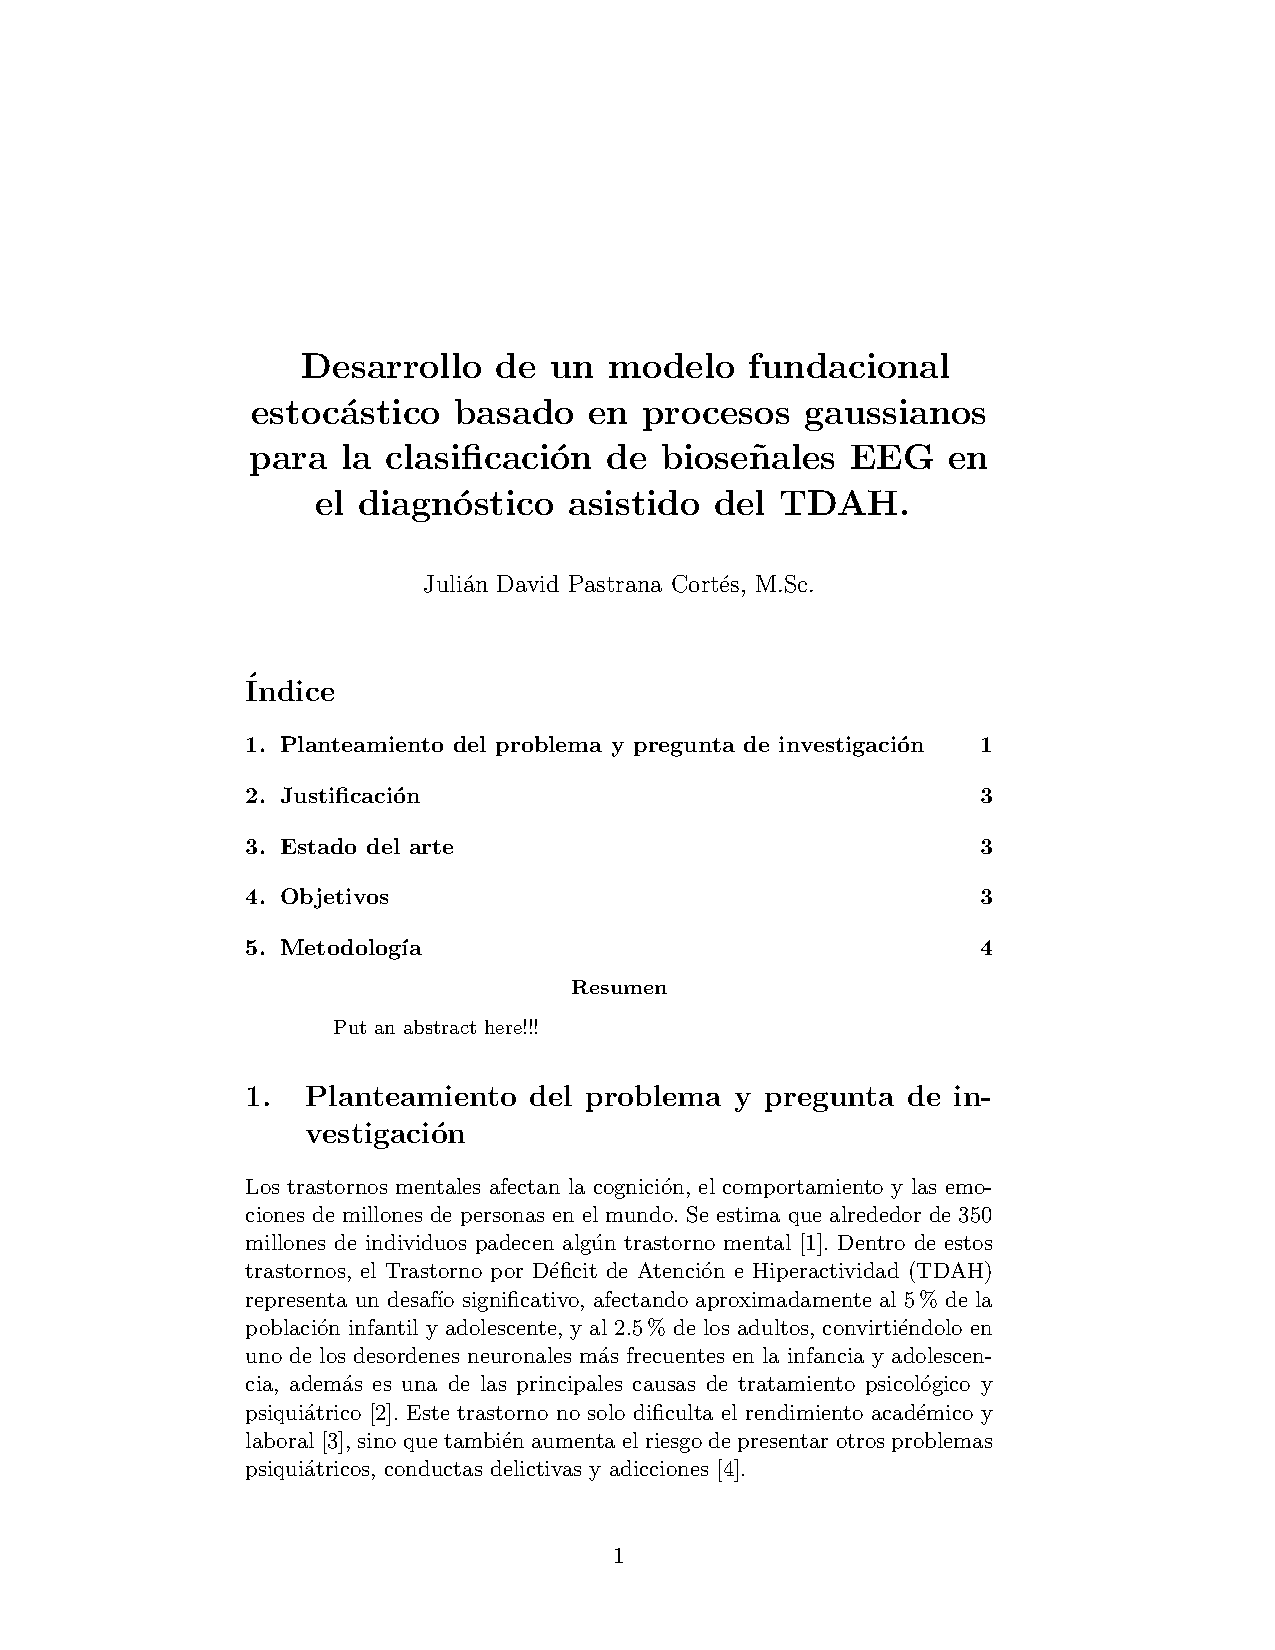
\includepdf[pages=1,
pagecommand={%
	\thispagestyle{plain}
		\Large\bfseries Propuesta doctorado
}
]{../propuesta_doctorado/main.pdf}
% Include remaining pages without any overlay
\includepdf[pages=2-last, pagecommand={}]{../propuesta_doctorado/main.pdf}

	\bibliographystyle{apalike}
	\bibliography{refs}
	
\end{document}
